\documentclass[11pt]{scrartcl}
\usepackage{evan}
\title{HW4}
\author{People}
\date{Date}
\definecolor{palegreen}{rgb}{0.6, 0.98, 0.6}
\begin{document}
\maketitle
\begin{problem}[\textcolor{red}{Some (counter)-example}]\phantom{0}

    \begin{enumerate}[(i)]
        \item Give an example of a finite graded poset $P$ with the Sperner property, together with a group $G$ acting on $P$, such that $P/G$ is \textit{not} Sperner.
        \item Consider the poset $P$ whose Hasse diagram is given by
        \begin{center}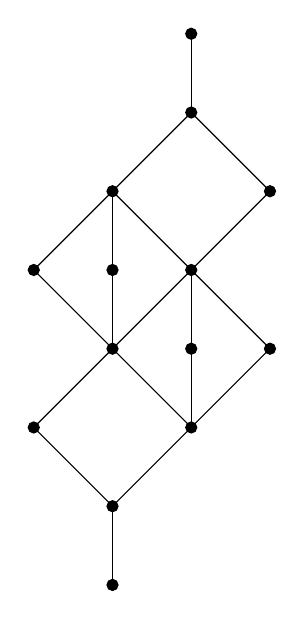
\begin{tikzpicture}
            \draw[fill=black] (0,-0.5) circle (2pt);
            \draw[fill=black] (0,0.5) circle (2pt);
            \draw[fill=black] (-1,1.5) circle (2pt);
            \draw[fill=black] (1,1.5) circle (2pt);
            \draw[fill=black] (0,2.5) circle (2pt);
            \draw[fill=black] (1,2.5) circle (2pt);
            \draw[fill=black] (2,2.5) circle (2pt);
            \draw[fill=black] (-1,3.5) circle (2pt);
            \draw[fill=black] (0,3.5) circle (2pt);
            \draw[fill=black] (1,3.5) circle (2pt);
            \draw[fill=black] (0,4.5) circle (2pt);
            \draw[fill=black] (2,4.5) circle (2pt);
            \draw[fill=black] (1,5.5) circle (2pt);
            \draw[fill=black] (1,6.5) circle (2pt);
            
            \draw (0,-0.5) -- (0,0.5);
            \draw (0,0.5 ) -- (-1,1.5);
            \draw (0,0.5) -- (1,1.5);
            \draw (1,1.5) -- (0,2.5);
            \draw (1,1.5) -- (1,2.5);
            \draw (1,1.5) -- (2,2.5);
            \draw (-1,1.5) -- (0,2.5);
            \draw (0,2.5) -- (-1,3.5);
            \draw (0,2.5) -- (0,3.5);
            \draw (0,2.5) -- (1,3.5);
            \draw (1,2.5) -- (1,3.5);
            \draw (2,2.5) -- (1,3.5);
            \draw (1,3.5) -- (0,4.5);
            \draw (1,3.5) -- (2,4.5);
            \draw (-1,3.5) -- (0,4.5);
            \draw (0,3.5) -- (0,4.5);
            \draw (0,4.5) -- (1,5.5);
            \draw (2,4.5) -- (1,5.5);
            \draw (1,5.5) -- (1,6.5);
            \end{tikzpicture}
            \end{center}
            Find a subgroup $G$ of $S_7$ such that $P\cong B_7/G$ or else prove that such a group does not exist.
    \end{enumerate}
\end{problem}
\begin{proof}
    \begin{enumerate}[(i)]
        \item We draw a Hasse diagram for $P$:
        \begin{center}
            \begin{asy}
                size(4cm);
                pair A=(0,0),B=(1,0),C=(2,0),D=(3,0),E=(4,0),AA=(0,1),BB=(1,1),CC=(2,1),DD=(3,1),EE=(4,1);
                dot(A);dot(B);dot(C);dot(D);dot(E);dot(AA);dot(BB);dot(CC);dot(DD);dot(EE);
                draw(A--AA);draw(B--BB);draw(C--CC);draw(D--DD);draw(E--EE);
                label("$1$",AA,N);
                label("$2$",BB,N);
                label("$3$",CC,N);
                label("$4$",DD,N);
                label("$5$",EE,N);
                label("$6$",A,S);
                label("$7$",B,S);
                label("$8$",C,S);
                label("$9$",D,S);
                label("$10$",E,S);
            \end{asy}
        \end{center}
        We see that $P$ is Sperner by inspection; its largest antichain is of length four, and each rank has four elements. Let $G=((1, 2, 3), (8, 9, 10))$ be the group generated by the permutations $(1,2,3)$ and $(8,9,10)$. By drawing the Hasse diagram of $P/G$, we see that is clearly not Sperner:
        \begin{center}
            \begin{asy}
                size(4cm);
                pair A=(1,0),B=(2,0),C=(2,0),D=(3,0),BB=(2,1),CC=(2,1),DD=(3,1),EE=(4,1);
                dot(A);dot(C);dot(D);dot(BB);dot(CC);dot(DD);dot(EE);
                draw(A--BB);draw(C--BB);draw(D--CC);draw(D--DD);draw(D--EE);
                label("$1,2,3$",CC,N);
                label("$4$",DD,N);
                label("$5$",EE,N);
                label("$6$",A,S);
                label("$7$",B,S);
                label("$8,9,10$",D,S);
            \end{asy}
        \end{center}
        \item %define our subgroup $G$ to be the permutations $\hat\pi$ induced by automorphisms $\pi\in S_7$, where $\hat\pi\{i,j\}=\{\pi\cdot i,\pi\cdot j\}$. Then, $P$ is the Hasse diagram identical to the poset of nonisomorphic simple graphs with $7$ vertices. We can see that $P\cong B_7/G$ by labelling the vertices, with much pain:
        \begin{center}
            \begin{asy}
                pair A = (0,-0.5), B = (0,0.5), C = (-1,1.5), D = (1,1.5), E = (0,2.5), F = (1,2.5), G = (2,2.5), H = (-1,3.5), I = (0,3.5), J = (1,3.5), K = (0,4.5), L = (2,4.5), M = (1,5.5), N = (1,6.5);

// Draw dots
dot(A); dot(B); dot(C); dot(D); dot(E); dot(F); dot(G); dot(H); dot(I); dot(J); dot(K); dot(L); dot(M); dot(N);

// Draw lines
draw(A--B); draw(B--C); draw(B--D); draw(D--E); draw(D--F); draw(D--G); draw(C--E); draw(E--H); draw(E--I); draw(E--J); draw(F--J); draw(G--J); draw(J--K); draw(J--L); draw(H--K); draw(I--K); draw(K--M); draw(L--M); draw(M--N);
            \end{asy}
        \end{center}
    \end{enumerate}
\end{proof}
\begin{problem}[\textcolor{red}{Binary Necklace Poset}]
    A $(0,1)$-\textit{necklace} of \textit{length} $n$ and \textit{weight} $i$ is a circular arrangement of $i$ $1$'s and $n-i$ $0$'s. For instance, the $(0,1)$-necklaces of length $6$ and weight $3$ are (writing a circular arrangement linearly) $000111, 001011, 010011$ and $010101$. Cyclic shifts of a linear word represent the same necklace.

    \begin{enumerate}[(i)]
        \item (easy) Show that $N_n$ is rank-symmetric, rank-unimodal and Sperner.
    \end{enumerate}
\end{problem}
\begin{proof}
    We have the same number of length $n$ necklaces of weight $i$ and $n-i$ because there is a bijection from simply flipping all digits. Thus, $p_i=p_{n-i}$, so $N_n$ is rank-symmetric. We can also calculate $p_i$ by first counting the $\binom n i$ necklaces with order and dividing by $n$ to account for cyclic shifts. Thus, \[p_i=\frac{1}{n}\binom n i ,\] so the unimodality of $N_n$ arises from the unimodality of the binomial coefficients. 
\end{proof}
\end{document}